\clearpage

\chapter{Sequenzdiagramme}
Sequenzdiagramme modellieren typische Szenarien eines Systems. Es wird die Kommunikation zwischen
Einheiten dargestellt.\\ \\
Folgende Use Cases wurden ausgewählt, um deren Kommunikation anhand von Sequenzdiagrammen darzustellen:\\
\begin{itemize}
  \item Spieler erstellen
  \item Spieler laden
  \item Spiel starten
\end{itemize}

\clearpage
\section{SD Spieler erstellen}
\begin{figure}[h!]
	\centering
    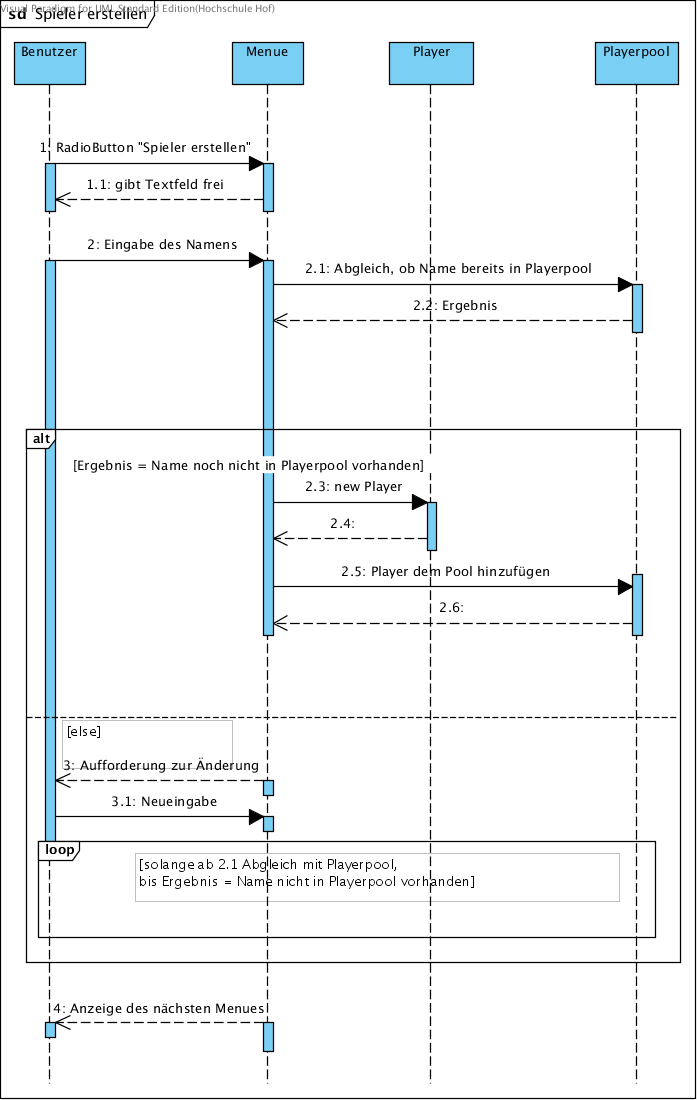
\includegraphics[width=13cm]{./SD_Spieler_erstellen.png}
	\label{layout_gesamt}
\end{figure}
\subsection{Beschreibung}
Der Benutzer wählt den Radio Button ,,Spieler erstellen''. Das Menue gibt das zugehörige Textfeld zur Eingabe des Namens frei. Nach Eingabe des Namens erfolgt ein Abgleich mit dem Playerpool, ob bereits ein Spieler unter diesem Namen gespeichert ist. Das Ergebnis wird zurück zur Klasse Menue geliefert. Ergibt die Prüfung, dass der Name noch nicht vorhanden ist, wird ein neues Objekt vom Typ Player erzeugt und anschließend dem Playerpool hinzugefügt. Ist der eingegebene Name bereits im Playerpool vorhanden, wird der Benutzer aufgefordert, einen anderen Namen einzugeben. Die Prüfung und Neueingabe erfolgt so lange, bis die Prüfung das Ergebnis = noch nicht im Playerpool vorhanden, liefert. Abschließend wird die nächste Menueseite angezeigt.

\clearpage
\section{SD Spieler laden}
\begin{figure}[h!]
	\centering
    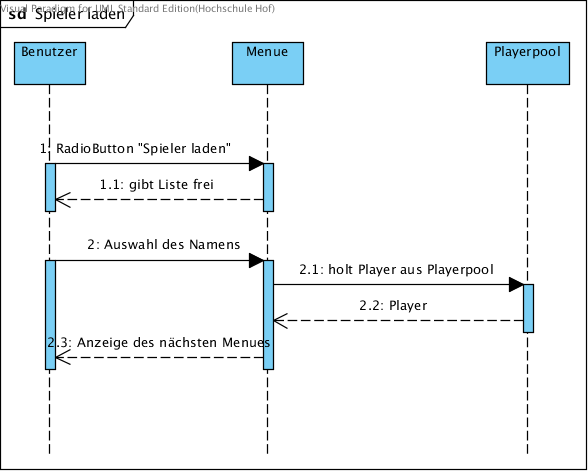
\includegraphics[width=\textwidth]{./SD_Spieler_laden.png}
	\label{layout_gesamt}
\end{figure}
\subsection{Beschreibung}
Der Benutzer klickt den Radio Button ,,Spieler laden'' an. Daraufhin wird durch die Klasse Menue eine Liste der gespeicherten Spieler als Dropdown-Liste freigegeben. Daraus kann der Benutzer den gewünschten Namen wählen. Das Menue nimmt die Auswahl entgegen und holt sich den entsprechenden Player aus dem Playerpool. Anschließend wird die nächste Maske angezeigt.

\clearpage
\section{SD Spiel starten}
\begin{figure}[h!]
	\centering
    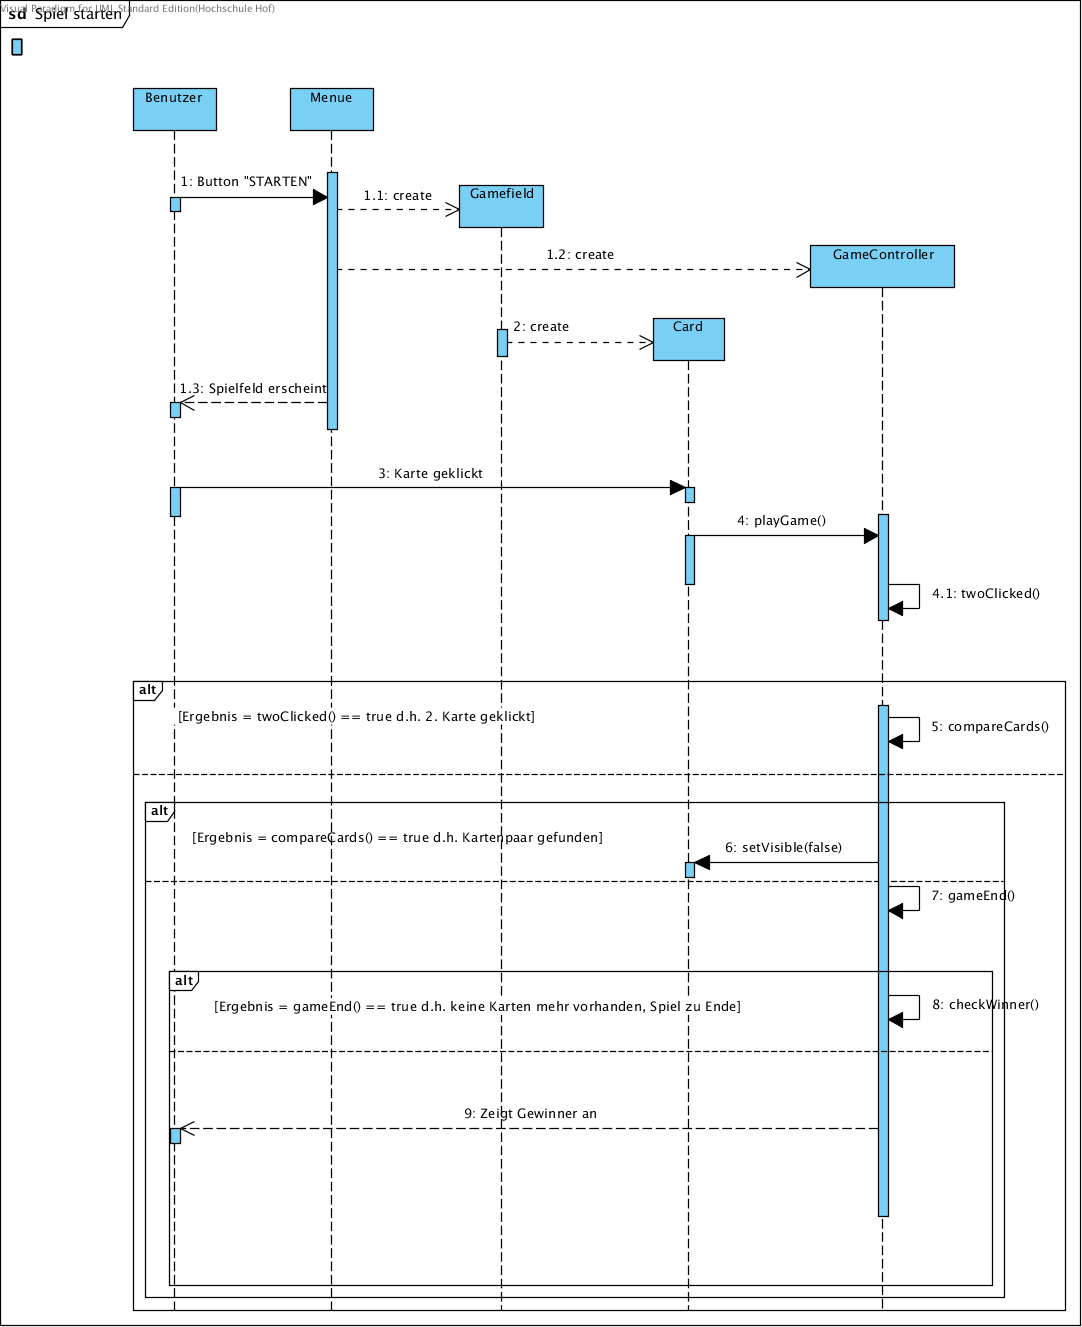
\includegraphics[width=15cm]{./SD_Spiel_starten.png}
	\label{layout_gesamt}
\end{figure}
\subsection{Beschreibung}
Der Benutzer drückt den Button ,,STARTEN``. Daraufhin werden von der Klasse Menue die Klassen GameField und GameController erstellt. Von GameField wird die Klasse Card erstellt. Hier werden die von der Klasse Menue übergebenen Parameter zum Erstellen des Spielfelds verarbeitet und die Karten gemischt. Anschließend wird dem Benutzer das Spielfeld angezeigt. Vom Benutzer wird eine Karte angeklickt. Dies wird in der Klasse Card aufgenommen und durch den Aufruf der Methode playGame() an den GameController weitergegeben. Der GameController ruft die Methode twoClicked() auf. Ist das Ergebnis true, wird die Methode compareCards() aufgerufen. Hat die Prüfung ergeben, dass die Karten übereinstimmen, werden die jeweiligen Karten mit der Methode setVisible(false) unsichtbar gemacht. Anschließend wird geprüft, ob das Spiel zu Ende ist. Trifft dies zu, wird die Methode checkWinner() aufgerufen und der hiermit ermittelte Gewinner dem Benutzer angezeigt. 





